\section{Dataset Realization}
%{\bf (*VP* se sposti la sez 1.7, devi distinguere fra il dataset dei dati originali e quello ottenuto dalla loro lavorazione. Il primo potrebbe essere "Original Dataset"}

For the creation of a dataset taht can be passed directly to our imputation models, we devised a procedure that
allowed us to merge all the original files into a single file, where for
each timestamp, we have all the data for the entire system at
that exact moment. Below is the final structure of the dataset
and the algorithm for generating it.

%Per la realizzazione del nostro dataset abbiamo ideato 
%una procedura che ci ha permesso di ottenere un unico file,
%in formato csv, dove, per ogni time stamp abbiamo tutti i dati
%di tutto l'impianto in quell'esatto istante. Di seguito 
%la struttira finale del dataset e l'algoritmo per generarlo.


\begin{table}[H]
	\begin{center}
		\begin{tabular}[c]{l|l|l|l}
			%\hline
			\multicolumn{1}{c|}{\textbf{timestamp}}              &
			\multicolumn{1}{c|}{\textbf{DEV.NAME$_1$\_FEAT$_1$}} &
			\multicolumn{1}{c|}{$\ldots$}                        &
			\multicolumn{1}{c}{\textbf{DEV.NAME$_n$\_FEAT$_n$}}                                   \\
			\hline

			01/10/2022 10:00                                     & $\ldots$ & $\ldots$ & $\ldots$ \\
			01/10/2022 10:05                                     & $\ldots$ & $\ldots$ & $\ldots$ \\
			01/10/2022 10:10                                     & $\ldots$ & $\ldots$ & $\ldots$ \\
			%\hline
		\end{tabular}
	\end{center}
	\caption{Final dataset feature structure.}\label{tab:datasetform}
\end{table}

\begin{algorithm}[H]
	\caption{Dataset aggregation algorithm}\label{alg:dataset}
	\begin{algorithmic}
		\Require data\_folder
		\Ensure \texttt{data\_folder} exists
		\State dev\_types $\gets$ find all file types inside \texttt{data\_folder} (e.g. meter, inverter, $\ldots$)
		\State dev\_content $\gets$ a dictionary with \texttt{dev\_types} types as $keys$ and empty $values$

		\For {\textbf{each} key \textbf{in} dev\_conent.keys}
		\State files $\gets$ find all file matching type \texttt{key} inside \texttt{data\_folder}
		\State sort \texttt{files} by date (asc.)
		\State temp\_type\_aggregate $\gets$ and empty csv table
		\For {\textbf{each} file \textbf{in} files}
		\State append all \texttt{file} lines to \texttt{temp\_type\_aggregate} table
		\EndFor
		\State dev\_content[key] $\gets$ temp\_type\_aggregate
		\EndFor
		\State\Comment{At this time we have a dictionary mapping a file type with all its available data}
		\State
		\State dataset $\gets$ an empty csv table
		\For {\textbf{each} type, data \textbf{in} dev\_content} \Comment{\texttt{type} is $key$, \texttt{data} is $value$}
		\State rename all \texttt{data} $columns$ to \texttt{data.deviceID}\_\texttt{$column$.name}
		\State except for 'timestamp' $column$
		\State dataset $\gets$ \texttt{dataset} and \texttt{data} tables using 'timestamp' column
		\EndFor
		\State save \texttt{dataset} table to file
	\end{algorithmic}
\end{algorithm}

\begin{table}[H]
	\begin{center}
		\begin{tabular}[c]{l|l|l|l}
			%\hline
			\multicolumn{1}{c|}{\textbf{timestamp}}      &
			\multicolumn{1}{c|}{\textbf{INV01\_PowerAC}} &
			\multicolumn{1}{c|}{\textbf{$\ldots$}}       &
			\multicolumn{1}{c}{\textbf{Cont\_TotalEnergy}}                                 \\
			\hline
			2022-02-02 00:05:00                          & NaN      & $\ldots$ & NaN       \\
			2022-02-02 00:10:00                          & NaN      & $\ldots$ & NaN       \\
			$\ldots$                                     & $\ldots$ & $\ldots$ & $\ldots$  \\
			2022-06-22 10:20:00                          & 175.66   & $\ldots$ & 8900941.5 \\
			2022-06-22 10:25:00                          & 178.29   & $\ldots$ & 8900995.5 \\
			2022-06-22 10:30:00                          & 180.82   & $\ldots$ & 8901036.0 \\
			$\ldots$                                     & $\ldots$ & $\ldots$ & $\ldots$  \\
			2023-06-16 18:00:00                          & NaN      & $\ldots$ & NaN       \\
			2023-06-16 18:05:00                          & NaN      & $\ldots$ & NaN       \\
		\end{tabular}
	\end{center}
	\caption{Some data from dataset after running Algorithm~\ref{alg:dataset}}\label{tab:datasetfinalvalues}
\end{table}

\subsection{Timestamp cyclical encoding}
To enable the models to learn the alternation of minutes, days,
and months as effectively as possible during the training phase,
we applied a procedure to transform each individual timestamp into
a pair of sine and cosine values, thus performing a cyclic
encoding of various seasonalities.

%Per permettere ai modelli, durante la fase di allenamento, di apprendere
%al meglio possibile l'alternarsi dei minuti, giorni e mesi abbiamo
%applicato una procedura per trasfrormare ogni signolo timestamp
%in una coppia di valori seno-coseno effettuando così un 
%encoding ciclico delle varie stagionalità.


\begin{algorithm}[H]
	\caption{Cyclical Encoding Algorithm}\label{alg:cyclicencoding}
	\begin{algorithmic}
		\Require dataset table
		\Ensure \texttt{dataset} \textbf{is not} empty
		\State dataset['minute\_sin'] $\gets \sin(2 \pi (\frac{\text{\texttt{dataset.timestamp.minute}}}{60}))$
		\State dataset['minute\_cos'] $\gets \cos(2 \pi (\frac{\text{\texttt{dataset.timestamp.minute}}}{60}))$


		\State dataset['hour\_sin'] $\gets \sin(2 \pi (\frac{\text{\texttt{dataset.timestamp.hour}}}{24}))$
		\State dataset['hour\_cos'] $\gets \cos(2 \pi (\frac{\text{\texttt{dataset.timestamp.hour}}}{24}))$


		\State dataset['day\_sin'] $\gets \sin(2 \pi (\frac{\text{\texttt{dataset.timestamp.day}}}{31}))$
		\State dataset['day\_cos'] $\gets \cos(2 \pi (\frac{\text{\texttt{dataset.timestamp.day}}}{31}))$

		\State dataset['month\_sin'] $\gets \sin(2 \pi (\frac{\text{\texttt{dataset.timestamp.month}}}{12}))$
		\State dataset['month\_cos'] $\gets \cos(2 \pi (\frac{\text{\texttt{dataset.timestamp.month}}}{12}))$
	\end{algorithmic}
\end{algorithm}

\begin{figure}[H]
	\centering
	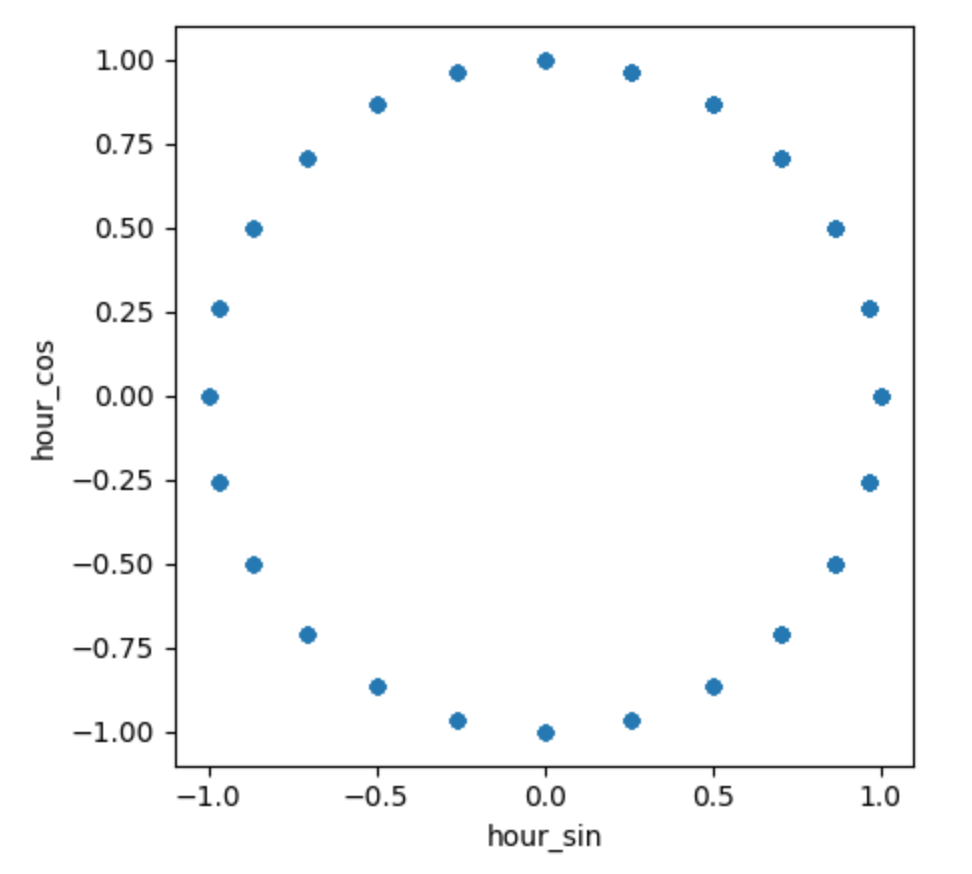
\includegraphics[width=0.7\linewidth, keepaspectratio]{chapters/2_data_preprocessing/imgs/hoursincosplot.png}
	\caption{Hour cyclical encoding plot.}\label{fig:encodingplot}
\end{figure}

\subsection{Historical weather}
In addition to the information from Solargis (see Section~\ref{sec:solargis}),
the models may require other weather data, such as cloud cover, rainfall, etc.
Therefore, we made an API call to Open-Meteo servers (see Section~\ref{sec:openmeteo}), using the \textquote{Historical Weather} functionality, to obtain the accurate past
forecasts for the time period covered by our dataset (from 02-02-2022 to 18-06-2023).

%Oltre alle infomazioni provenienti da Solargis
%(vedi Sezione \ref{sec:solargis}), i modelli potrebbero avere bisogno
%di altri dati meteo, come la presenza di nuvole, pioggia, ecc.
%Abbiamo quindi effettuato una chiamata API ai server di Open-Meteo (vedi
%Sezione \ref{sec:openmeteo}), usando la funzionalità
%\textquote{Historical Weather}, per ottenere le previsioni passate
%esatte del periodo temporale che copre il nostro dataset (dal 02-02-2022 al 18-06-2023).

\begin{algorithm}[H]
	\caption{Open-Meteo data request Algorithm}\label{alg:openemeteo}
	\begin{algorithmic}
		\Require dataset table
		\Ensure \texttt{dataset} \textbf{is not} empty

		\State meteo\_data $\gets$ require meteo feature from Open-Mete public API
		\State dataset $\gets$ merge \texttt{dataset} and \texttt{meteo\_data} tables using \texttt{timestamp} column

		\State
		\State /* At this time we have \texttt{dataset} timestamps as 5 minute frequency and \texttt{meteo\_data} as 1 hour frequency. */
		\State

		\State use a \textit{forward fill} method to fill gaps inside \texttt{dataset} table only for \texttt{meteo\_data} columns.
	\end{algorithmic}
\end{algorithm}

We have obtained most of the information made available by Open-Meteo since the API
request is free \cite{openmeteo} and computationally and storage-wise inexpensive.
These will be filtered at a later time (see Section~\ref{sec:featureselection}).
Among these, we find \texttt{sunrise} and \texttt{sunset}, which indicate the exact time
(down to the minute) of when dawn and sunset occurred, respectively.
These two features will be used to create a new column in our dataset called
\texttt{is\_day}, which will allow the model to understand whether it is
analyzing a period of time during the day or night.
This is to ensure that it does not make energy production predictions
during the night.

%Abbiamo preso la maggior parte delle informazioni messe a disposizione 
%da Open-Meteo dato che la richiesta API è gratuita e poco costosa a
%livello computazionale e di archiviazione. Queste verranno poi filtrate in un
%momento successivo (vedi Sezione \ref{sec:featureselection}).
%Tra queste troviamo \texttt{sunrise} e \texttt{sunset} che stanno
%ad indicare rispettivamente l'ora esatta (con precisione al minuto) di
%quando è avvenuta l'alba e l'ora esatta (con precisione al minuto) di
%quando è avvenuto il tramonto. Queste due feature ci serviranno per 
%costruire una nuova colonna nel nostro dataset, denominata \texttt{is\_day}, che permetterà al modello di comprendere se sta analizzando un
%periodo di tempo dove è giorno o nette. Questo per assicurarci che
%non daranno come predizioni produzioni di energia duarante la notte.

%\newpage
\begin{longtable}[c]{p{0.3\linewidth}|p{0.07\linewidth}| p{0.54\linewidth}}
	\hline
	\multicolumn{1}{c|}{\textbf{Feature}}                                                                                                                                                   &
	\multicolumn{1}{c|}{\textbf{Unit}}                                                                                                                                                      &
	\multicolumn{1}{c}{\textbf{Note}}                                                                                                                                                                                                                                                                                                                                                                                                                                                                                          \\
	\hline
	\verb|temperature_2m|                                                                                                                                                                   & °C                      & Air temperature at 2 meters above ground.                                                                                                                                                                                                                                                              \\
	\verb|relativehumidity_2m|                                                                                                                                                              & \%                      & Relative humidity at 2 meters above ground.                                                                                                                                                                                                                                                            \\
	\verb|dewpoint_2m|                                                                                                                                                                      & °C                      & Dew point temperature at 2 meters above ground. The dew point of a given body of air is the temperature to which it must be cooled to become saturated with water vapor. This temperature depends on the pressure and water content of the air.                                                        \\ %% preso da: https://en.wikipedia.org/wiki/Dew_point
	\verb|apparent_temperature|                                                                                                                                                             & °C                      & Apparent temperature is the perceived feels-like temperature combining wind chill factor, relative humidity and solar radiation.                                                                                                                                                                       \\
	\verb|precipitation|                                                                                                                                                                    & mm                      & Total precipitation (rain, showers, snow) sum of the preceding hour. Data is stored with a 0.1 mm precision. If precipitation data is summed up to monthly sums, there might be small inconsistencies with the total precipitation amount.                                                             \\
	\verb|weathercode|                                                                                                                                                                      & wmo                     & Weather condition as a numeric code. Follow WMO weather interpretation codes. Weather code is calculated from cloud cover analysis, precipitation and snowfall. As barely no information about atmospheric stability is available, estimation about thunderstorms is not possible.                     \\
	\verb|pressure_msl| \verb|surface_pressure|                                                                                                                                             & hPa                     & Atmospheric air pressure reduced to mean sea level (msl) or pressure at surface. Typically pressure on mean sea level is used in meteorology. Surface pressure gets lower with increasing elevation.                                                                                                   \\

	\verb|cloudcover| 	Instant                                                                                                                                                              & \%                      & Total cloud cover as an area fraction.                                                                                                                                                                                                                                                                 \\

	\verb|et0_fao_| \verb|evapotranspiration|                                                                                                                                               & mm                      & $ET_0$ Reference Evapotranspiration of a well watered grass field. Based on FAO-56 Penman-Monteith equations $ET_0$ is calculated from temperature, wind speed, humidity and solar radiation. Unlimited soil water is assumed. $ET_0$ is commonly used to estimate the required irrigation for plants. \\
	\verb|vapor_pressure_| \verb|deficit|                                                                                                                                                   & kPa                     & Vapor Pressure Deificit (VPD) in kilopascal (kPa). For high VPD (>1.6), water transpiration of plants increases. For low VPD (<0.4), transpiration decreases.                                                                                                                                          \\
	\verb|windspeed_10m| \verb|windspeed_100m|                                                                                                                                              & km/h                    & Wind speed at 10 or 100 meters above ground. Wind speed on 10 meters is the standard level.                                                                                                                                                                                                            \\
	\verb|winddirection_10m| \verb|winddirection_100m|                                                                                                                                      & °                       & Wind direction at 10 or 100 meters above ground.                                                                                                                                                                                                                                                       \\
	\verb|windgusts_10m |                                                                                                                                                                   & km/h                    & Gusts at 10 meters above ground of the indicated hour. Wind gusts in CERRA are defined as the maximum wind gusts of the preceding hour.                                                                                                                                                                \\ %Please consult the ECMWF IFS documentation for more information on how wind gusts are parameterized in weather models.\\
	\verb|soil_temperature_0_| \verb|   to_7cm| \verb|soil_temperature_7_| \verb|   to_28cm| \verb|soil_temperature_28_| \verb|   to_100cm| \verb|soil_temperature_100_| \verb|   to_255cm| & °C                      & Average temperature of different soil levels below ground.                                                                                                                                                                                                                                             \\
	                                                                                                                                                                                        &                         &                                                                                                                                                                                                                                                                                                        \\
	\verb|soil_moisture_0_| \verb|   to_7cm| \verb|soil_moisture_7_| \verb|   to_28cm| \verb|soil_moisture_28_| \verb|   to_100cm| \verb|soil_moisture_100_| \verb|   to_255cm|             & $\text{m}^3/\text{m}^3$ & Average soil water content as volumetric mixing ratio at 0-7, 7-28, 28-100 and 100-255 cm depths.                                                                                                                                                                                                      \\
	\caption{All feature selected from Open-Meteo with description\cite{openmeteo}.}\label{tab:openmeteofeatures}
\end{longtable}
\newpage
The new feature \texttt{is\_day} contains two values: 0 and 1,
representing \textit{Night} and \textit{Day}, respectively.
To create this feature, we add 0 with a frequency of 5 minutes until sunrise,
then add 1 until sunset, and finally add more 0s until the end of the day.
We repeat this process for each day in the dataset to create a new column that,
for each timestamp, will indicate whether it is day or night.

%La nuova feature \texttt{is\_day} conterrà due valori 0 e 1 che rappresenteranno 
%rispettivamente \textit{Notte} e \textit{Giorno}. Per la creazione di questa feature
%aggiungiamo 0, con frequenza di 5 minuit, fin all'ora dell'alba, poi degli 1 fino al
%tramonto e poi altri 0 fino alla fine del giorno. Ripetiamo questa operazione per tutti
%i giorni del dataset così da ottenere una nuova colonna che, per ogni timestamp, ci dirà se è giorno o notte.

\begin{algorithm}[H]
	\caption{is\_day feature generation Algorithm}\label{alg:isday}
	\begin{algorithmic}
		\Require dataset table, sunrise and sunset table
		\Ensure \texttt{dataset} \textbf{is not} empty, \texttt{sunrise} and \texttt{sunset} tables \textbf{match} \texttt{dataset} days

		\State is\_day $\gets$ empty table column
		\For{\textbf{each} day \textbf{in} dataset.days}
		\State temp\_is\_day $\gets$ empty table column
		\State day\_start $\gets$ sunrise[day] \Comment{get sunrise timestamp for that day}
		\State day\_start $\gets$ find the nearest \texttt{dataset.timestamp} to \texttt{day\_start}

		\State day\_end $\gets$ sunset[day]
		\State day\_end $\gets$ find the nearest \texttt{dataset.timestamp} to \texttt{day\_end}
		\State /* if \texttt{sunrise[day] = 7:04} then \texttt{day\_start = 7:05} */
		\State
		\State /* 0 means Night, 1 mean Day */
		\State temp\_is\_day $\gets$ add 0s starting from 00:00 to \texttt{day\_start}

		as 5 minute frequency
		\State temp\_is\_day $\gets$ add 1s starting from \texttt{day\_start} to \texttt{day\_end}

		as 5 minute frequency
		\State temp\_is\_day $\gets$ add 0s starting from \texttt{day\_end} day end

		as 5 minute frequency
		\State \textbf{append} to \texttt{is\_day} column \texttt{temp\_is\_day} values
		\EndFor
		\State \textbf{merge} \texttt{is\_day} column to \texttt{dataset} table
	\end{algorithmic}
\end{algorithm}

%\begin{lstlisting}[captionpos=b, caption=HTTP GET request to Open-Meteo API.]
%GET / HTTP/1.1 
%Host: archive-api.open-meteo.com/v1/archive  
%
%latitude=...&longitude=...&
%start_date=2022-02-02&
%end_date=2023-06-18&
%
%hourly=temperature_2m,relativehumidity_2m,dewpoint_2m,
%       apparent_temperature,precipitation,weathercode,
%       pressure_msl,surface_pressure,cloudcover,
%       et0_fao_evapotranspiration,
%       vapor_pressure_deficit,windspeed_10m,
%       windspeed_100m,winddirection_10m,
%       winddirection_100m,windgusts_10m,
%       soil_temperature_0_to_7cm,soil_temperature_7_to_28cm,
%       soil_temperature_28_to_100cm,
%       soil_temperature_100_to_255cm,
%       soil_moisture_0_to_7cm,soil_moisture_7_to_28cm,
%       soil_moisture_28_to_100cm,soil_moisture_100_to_255cm&
%
%daily=sunrise,sunset&
%timezone=Europe%2FBerlin
%
%\end{lstlisting}

\subsection{Dealing with gaps}

\begin{figure}[H]
	\centering
	\begin{subfigure}[t]{0.48\textwidth}
		\centering
		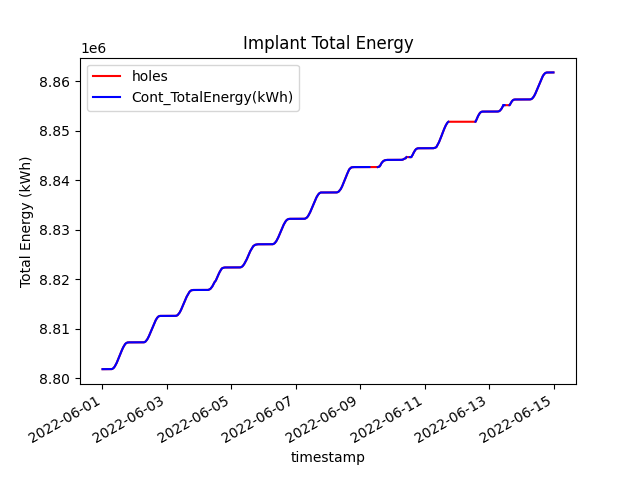
\includegraphics[width=\textwidth, keepaspectratio]{chapters/2_data_preprocessing/imgs/totenergybuco1.png}
	\end{subfigure}
	\hspace{0.1cm}
	\begin{subfigure}[t]{0.48\textwidth}
		\centering
		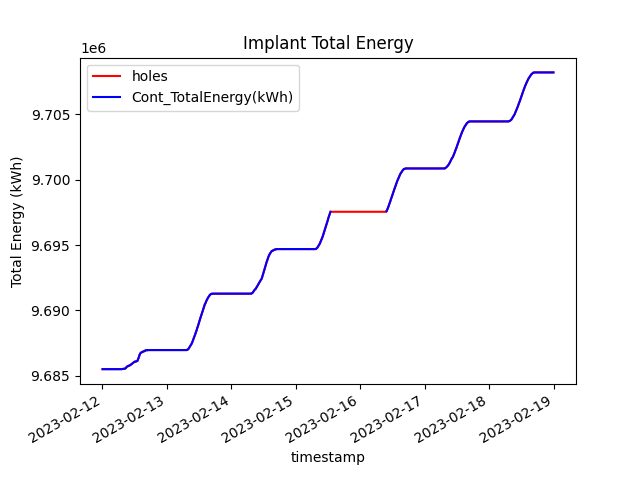
\includegraphics[width=\textwidth, keepaspectratio]{chapters/2_data_preprocessing/imgs/totenergybuco2.png}
	\end{subfigure}\\

	\begin{subfigure}[t]{0.48\textwidth}
		\centering
		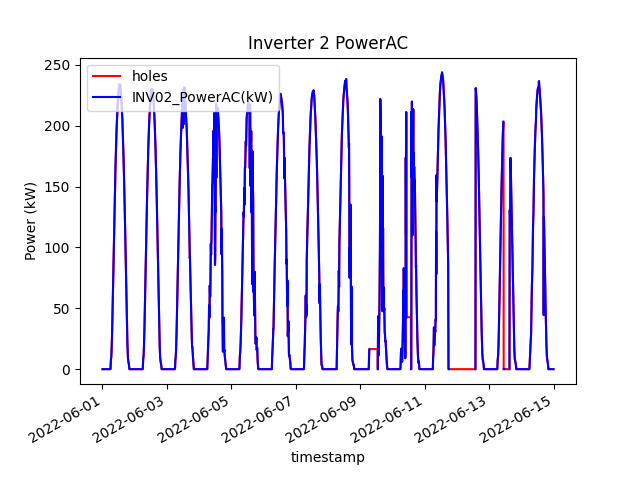
\includegraphics[width=\textwidth, keepaspectratio]{chapters/2_data_preprocessing/imgs/inv02powerbuco1.png}
	\end{subfigure}
	\hspace{0.1cm}
	\begin{subfigure}[t]{0.48\textwidth}
		\centering
		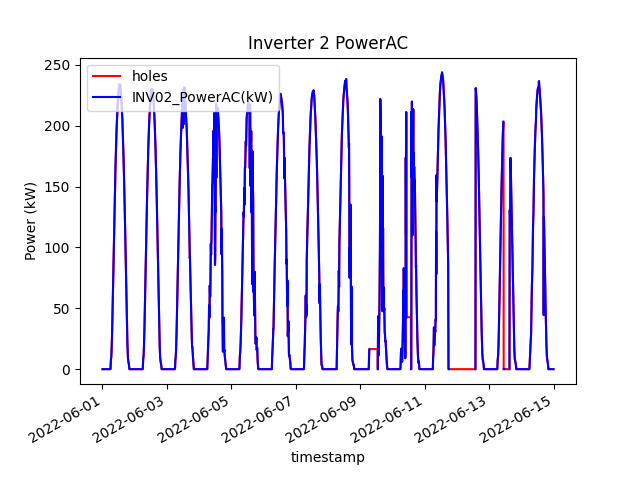
\includegraphics[width=\textwidth, keepaspectratio]{chapters/2_data_preprocessing/imgs/inv02powerbuco1.png}
	\end{subfigure}
	\caption{Some dataset \textquote{holes}. The charts at the top refer to the Implant's Total Energy, while those at the bottom refer to the Inverter 2's Power. The charts on the left range from 01-06-2022 to 15-06-2022, while those on the right range from 12-02-2023 to 19-02-2023.}\label{fig:graficibuchi}
\end{figure}

As we can see from Figure~\ref{fig:graficibuchi}, there are certain
periods within the dataset (highlighted in red) where data is missing,
which we refer to as \textquote{holes}. These data gaps can cause problems during model training
(hindering the correct calculation of the loss function), and therefore,
they need to be removed.

One possible approach for holes removal
is to perform a \textit{fill} operation: filling the gap with the
first available non-null value. This tactic may be considered
acceptable only if the time span involves just a few timestamps.
However, if we are talking about several hours or even days, it
significantly distorts the overall production and instantaneous
power trends, resulting, especially in very unfortunate cases, with extremely abnormal production curves.

The solution we have adopted to address this problem is the removal of
the entire day when a hole occurs. For example, if we have a data
gap from 12-02-2023 23:00 to 13-02-2023 10:40, the days
12-02-2023 and 13-02-2023 will be completely removed. With this
method, we lose some data, but as we will see later, the number of
gaps is not extremely high, and this data loss is not
debilitating. The following algorithm summarizes what has
just been described.

%Come possiamo vedere dalla Figura \ref{fig:graficibuchi}, all'interno del dataset sono presenti alcuni periodi (evidenziati in rosso) di assenza dati che è ciò che chiamiamo \textquote{buco}.
%Lasciare questi buchi causa problemi durante l'allenamento dei modelli (impediscono il corretto calcolo della loss function) e per questo
%vanno rimossi. Un possibile approccio per la loro rimozione è effettuare
%un'operazione di \textquote{fill}: riempio il buco con il primo valore non nullo disponibile.
%Questa tattica può essere ritenuta accettabile solo se il lasso di tempo coinvolge solo qualche timestamp, se invece parliamo di
%qualche ora o addirittura giorni questo va ad alterare notevolmente
%l'andamento della produzione totale e della potenza istantanea, risultando in casi molto sfortunati, ad avere curve di produzione estremamente anomale.
%
%La soluzione che abbiamo adottato per risolvere questo problema è
%l'eliminazione di tutto il giorno in cui si presenta il buco.
%Per fare un esempio pratico, se abbiamo un buco di dati che va dal
%12-02-2023 23:00 al 13-02-2023 10:40, verranno completamente eliminati
%i giorni 12-02-2023 e 13-02-2023. Con questo metodo andiamo a perdere 
%alcuni dati, ma come vedremo poi, il numero dei buchi non è estremamente
%elevato e la perdita di questi dati non risulta invalidante. Il seguente algoritmo riassume quanto appena detto.
%
\noindent\begin{minipage}[t]{0.55\linewidth}
	\begin{algorithm}[H]
		\caption{Holes Removal Algorithm.}\label{alg:holes}
		\begin{algorithmic}
			\Require dataset table
			\Ensure \texttt{dataset} \textbf{is not} empty

			\State holes $\gets$ find all timestamp from \texttt{dataset} table, where there are some \texttt{Nan}s inside the columns
			\For{\textbf{each} row \textbf{in} \texttt{dataset.rows}}
			\If {row.timestamp \textbf{is in} \texttt{holes}}
			\State drop \texttt{row} from \texttt{dataset} table
			\EndIf
			\EndFor
		\end{algorithmic}
	\end{algorithm}

\end{minipage}%
\hfill%
\begin{minipage}[t]{0.30\linewidth}
	\begin{table}[H]
		\centering
		\begin{tabular}[c]{l}
			\multicolumn{1}{c}{\textbf{Timestamp}} \\
			\hline
			2022-06-09                             \\
			2022-06-10                             \\
			2022-06-11                             \\
			2022-06-12                             \\
			2022-06-13                             \\
			2022-06-28                             \\
			2022-06-29                             \\
			2022-06-30                             \\
			2022-08-26                             \\
			2022-09-23                             \\
			2022-10-06                             \\
			2023-02-03                             \\
			2023-02-15                             \\
			2023-02-16                             \\
			2023-03-26                             \\
		\end{tabular}
		\caption{Timestamps deleted after running the Algorithm~\ref{alg:holes}}
	\end{table}
\end{minipage}

\subsection{Target Feature}
For the deep learning models that we will introduce later,
it could be very difficult learning how to predict the Total Missing Energy,
as it is a curve that grows constantly, potentially to infinity.
These models need to have features that vary within a limited range of
values. To achieve this, we transformed the variable
\verb|Cont_TotalEnergy(kWh)| from cumulative to instantaneous values of
produced energy, thereby limiting its values within a finite range.
This new feature was added to the dataset with the name \verb|target|.

%Per i modelli di deep learning che presenteremo successivamente, potrebbe
%risultare molto difficile imparare a prevedere l'Energia Totale mancante
%in quanto è una curva che cresce costantemente, potenzialmente all'infinito.
%Questi modelli hanno bisogno di avere features che variano in un range 
%limitato di valori. Per ottenere ciò abbiamo trasformato la variabile
%\verb|Cont_TotalEnergy(kWh)| da cumulata a valori istantanei di energia prodotta, andando così a limitare i suoi valori in un range finito. 
%Questa nuova feature è stata aggiunta al dataset con il nome di \verb|target|.

\begin{algorithm}[H]
	\caption{Cumulative Energy to Instant Energy Algorithm.}\label{alg:cumtoinstant}
	\begin{algorithmic}
		\Require dataset table
		\Ensure \texttt{dataset} \textbf{is not} empty

		\State target $\gets$ empty column
		\For{\textbf{each} (prev\_val, val) \textbf{in} dataset["Cont\_TotalEnergy(kWh)"]}
		\State diff $\gets \text{val} - \text{prev\_val}$
		\State \textbf{append} \texttt{diff} value to \texttt{target} column
		\EndFor
		\State /* Now we have target column with first value missing */
		\State /* We can add a 0 as fist value because its night time */
		\State \textbf{append} (in head) 0 to \texttt{target} column
		\State \textbf{merge} \texttt{target} and \texttt{dataset}
	\end{algorithmic}
\end{algorithm}

\begin{figure}[H]
	\centering
	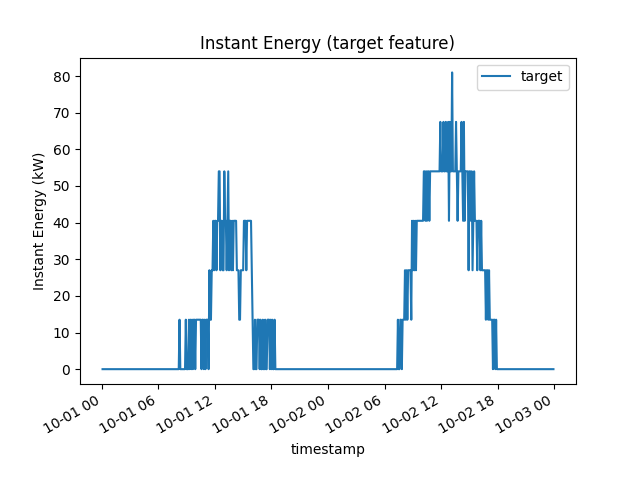
\includegraphics[width=\linewidth, keepaspectratio]{chapters/2_data_preprocessing/imgs/targetfeature.png}
	\caption{Instant Energy (\texttt{target} feature) 2 days plot.}\label{fig:targetfeature}
\end{figure}

\subsection{Re-Sampling}
Finally, after all the operations described above, we obtain a dataset
with samples taken at 5-minute intervals. As we can see from
Figure~\ref{fig:targetfeature}, this data appears to be quite noisy,
which could pose
challenges during the training phase. Moreover, most of the reports
provided by photovoltaic plant operators are at a 15-minute frequency.
To prevent potential issues and align with this standard, we have
written and applied a re-sampling procedure.

%Infine, dopo tutte le operazioni descritte in precedenza, ci troviamo con
%un dataset che ha campioni presi in intervalli di 5 minuti. Come possiamo
%vedere anche dalla Figura \ref{fig:targetfeature} questi dati risultano
%essere abbastanza rumorosi, ciò potrebbe portare a delle difficoltà 
%nella fase di addestramento. In più la maggiorpare dei report che vengono
%forniti dai gestori di impianti fotovoltaici sono ad una frequenza di 15 minuti. Per prevenire eventuali problemi ed adeguarci a questo standard
%abbiamo scritto ed applicato una procedura di Re-Sampling.
%

\begin{algorithm}[H]
	\caption{15 minute Re-Sampling Algorithm.}\label{alg:resampling}
	\begin{algorithmic}
		\Require dataset table
		\Ensure \texttt{dataset} \textbf{is not} empty

		\For{\textbf{each} feature \textbf{in} dataset.features}
		\If{feature \textbf{is} Cumulative}
		\State feature $\gets$ sample \texttt{feature} column using 15 min. sampling rate
		\Else
		\State feature $\gets$ aggregate values every 15 minutes and sum them to form a single value
		\EndIf
		\EndFor
	\end{algorithmic}
\end{algorithm}

\begin{figure}[H]
	\centering
	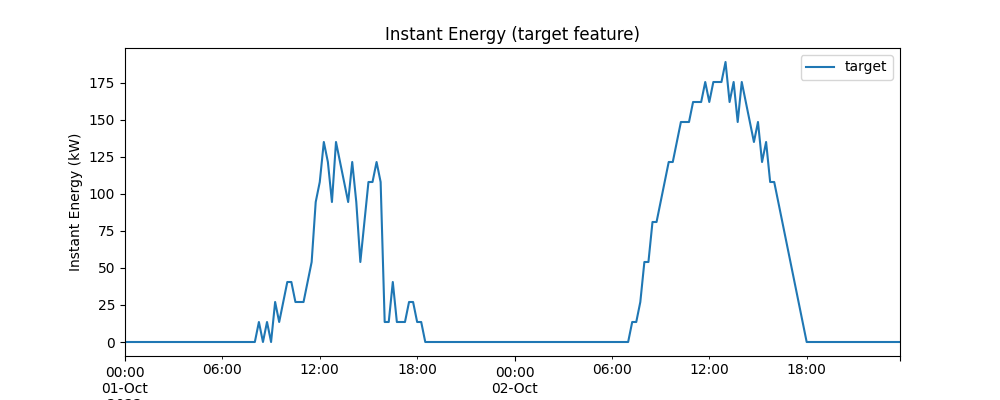
\includegraphics[width=\linewidth, keepaspectratio]{chapters/2_data_preprocessing/imgs/targetfeature15min.png}
	\caption{Instant Energy feature on 15 minute re-sampled dataset.}\label{fig:15min}
\end{figure}

